% Created 2017-12-20 Wed 11:49
\documentclass[presentation]{beamer}
\usepackage[utf8]{inputenc}
\usepackage[T1]{fontenc}
\usepackage{fixltx2e}
\usepackage{graphicx}
\usepackage{longtable}
\usepackage{float}
\usepackage{wrapfig}
\usepackage{rotating}
\usepackage[normalem]{ulem}
\usepackage{amsmath}
\usepackage{textcomp}
\usepackage{marvosym}
\usepackage{wasysym}
\usepackage{amssymb}
\usepackage{hyperref}
\tolerance=1000
\usepackage{graphicx} \DeclareMathOperator{\argmin}{argmin}
\usetheme{simple}
\usecolortheme{}
\usefonttheme{serif}
\useinnertheme{}
\useoutertheme{}
\author{Talon Chandler}
\date{December 20, 2017}
\title{Update On 3D Orientation Reconstruction}
\hypersetup{
  pdfkeywords={},
  pdfsubject={},
  pdfcreator={Emacs 25.3.1 (Org mode 8.2.10)}}
\begin{document}

\maketitle
\begin{frame}[label=sec-1]{Forward Model}
\begin{align*}
g_i = \int_{\mathbb{S}^2}d\hat{\textbf{r}}\ h_i(\hat{\textbf{r}})f_i(\hat{\textbf{r}})
\end{align*}
\begin{itemize}
\item $g_i$ $\rightarrow$ intensity measurement
\item $h_i$ $\rightarrow$ point response function
\item $f_i$ $\rightarrow$ orientation distribution function
\end{itemize}
\end{frame}
\begin{frame}[label=sec-2]{Fourier Transforms}
\begin{align*}
\text{Fourier Transform} \rightarrow F(\nu) &= \int_{\mathbb{R}}dx\ f(x)e^{-2\pi i x\nu}\\
\text{Spherical Fourier Transform} \rightarrow F_l^m &= \int_{\mathbb{S}^2}d\hat{\textbf{r}}\ f(\hat{\textbf{r}})\overline{Y_l^m(\hat{\textbf{r}})}\\
\end{align*}
\end{frame}
\begin{frame}[label=sec-3]{Forward Model}
\begin{align*}
g_i = \int_{\mathbb{S}^2}d\hat{\textbf{r}}\ h_i(\hat{\textbf{r}})f_i(\hat{\textbf{r}})
\end{align*}
Simplifies to:
\begin{align*}
g_i = \textbf{H}^T\textbf{F}
\end{align*}
\begin{itemize}
\item $\textbf{H}$ $\rightarrow$ is a vector of the Fourier coefficients of the point response function
\item $\textbf{F}$ $\rightarrow$ is a vector of the Fourier coefficients of the orientation distribution function
\end{itemize}
Multiple measurements:
\begin{align*}
\textbf{g} = \Psi\textbf{F}
\end{align*}
\end{frame}
\begin{frame}[label=sec-4]{No Prior Reconstruction}
\begin{align*}
\textbf{F} = \Psi^+\textbf{g}
\end{align*}
If $\Psi$ is full column rank then we can recover $\textbf{F}$---the spherical
harmonic coefficients passed by the system.\vspace{2em}

$\textbf{F}$ is a representation of the true object projected onto the spherical 
harmonic components passed by the system.
\end{frame}
\begin{frame}[label=sec-5]{Isotropic Excitation - Single Pixel $z$ View}
\begin{align*}
h(\theta, \phi) &= \sin^2\theta = \\ \\
\end{align*}
\begin{center}
\begin{tabular}{ccccccccc} 
&&&&$\frac{4\sqrt{\pi}}{3}Y_0^0$&&&&\\
&&&-&-&-&&&\\
&&-&-&$-4\frac{\sqrt{5\pi}}{15}Y_1^0$&-&-&&\\
&-&-&-&-&-&-&-&\\
-&-&-&-&-&-&-&-&-\\
\end{tabular}
\end{center}
\end{frame}
\begin{frame}[label=sec-6]{Isotropic Excitation - Single Pixel $x$ View}
\begin{align*}
h(\theta, \phi) &= 1 - \sin^2\theta\cos^2\phi= \\ \\
\end{align*}
\begin{center}
\begin{tabular}{ccccccccc} 
&&&&$\frac{4\sqrt{\pi}}{3}Y_0^0$&&&&\\
&&&-&-&-&&&\\
&&$-\frac{\sqrt{30\pi}}{15}Y_1^{-2}$&-&$+2\frac{\sqrt{5\pi}}{15}Y_1^0$&-&$-\frac{\sqrt{30\pi}}{15}Y_1^2$&&\\
&-&-&-&-&-&-&-&\\
-&-&-&-&-&-&-&-&-\\
\end{tabular}
\end{center}
\end{frame}

\begin{frame}[label=sec-7]{Isotropic Excitation - Single Pixel $y$ View}
\begin{align*}
h(\theta, \phi) &= 1 - \sin^2\theta\sin^2\phi= \\ \\
\end{align*}
\begin{center}
\begin{tabular}{ccccccccc} 
&&&&$\frac{4\sqrt{\pi}}{3}Y_0^0$&&&&\\
&&&-&-&-&&&\\
&&$\frac{\sqrt{30\pi}}{15}Y_1^{-2}$&-&$+2\frac{\sqrt{5\pi}}{15}Y_1^0$&-&$\frac{\sqrt{30\pi}}{15}Y_1^2$&&\\
&-&-&-&-&-&-&-&\\
-&-&-&-&-&-&-&-&-\\
\end{tabular}
\end{center}
\end{frame}
\begin{frame}[label=sec-8]{Isotropic Excitation - Single Pixel ($\Theta$, $\Phi$) View}
\small
\begin{align*}
h(\theta, \phi) &= 1 - (\sin\Theta\cos\Phi\sin\theta\cos\phi + \sin\Theta\sin\Phi\sin\theta\sin\phi + \cos\Theta\cos\theta)^2= \\
\end{align*}
\footnotesize
\begin{center}
\begin{tabular}{ccccc} 
$\frac{4\sqrt{\pi}}{3}Y_0^0$&&&&\\
-&-&&&\\
$+2\frac{\sqrt{5\pi}}{15}(3\sin^2\Theta - 2)Y_1^0$&$-\frac{2\sqrt{30\pi}}{15}\sin\Theta\cos\Theta e^{-i\phi} Y_1^{1}$&$-\frac{\sqrt{30\pi}}{15}\sin^2\Theta e^{-2i\phi} Y_1^{2}$&&\\
-&-&-&-&\\
-&-&-&-&-\\
\end{tabular}
\end{center}
\begin{itemize}
\item Need >=4 single pixel measurements to satisfy full rank condition. 
\item Choose orientations so that the spherical harmonic coefficients are measured as independently as possible. I expect a tetrahedron pattern is optimal, but I haven't shown this. 
\end{itemize}
\end{frame}

\begin{frame}[label=sec-9]{diSPIM - polarized illuminatation from z - detect from x - $\phi$$_{\text{p}}$ parameter}
\small
\begin{align*}
h(\theta, \phi) &= \sin^2\theta\cos^2(\phi - \phi_{\text{p}})\cdot2[A + B(\cos^2\theta + \sin^2\theta\sin^2\phi)] = 
\end{align*}
\tiny
\begin{center}
\begin{tabular}{ccccccccc} 
&&&&$H_0^0Y_0^0$&&&&\\
&&&-&-&-&&&\\
&&$+\overline{H_2^2}Y_2^{-2}$&-&+$H_2^0Y_2^0$&-&+$H_2^2Y_2^{2}$&&\\
&-&-&-&-&-&-&-&\\
$+\overline{H_4^4}Y_4^{-4}$&-&$+\overline{H_4^2}Y_4^{-2}$&-&$+H_4^0Y_4^0$&-&$+H_4^2Y_4^2$&-&$+H_4^4Y_4^4$\\
\end{tabular}
\end{center}
\begin{align*}
H_0^0 &= \frac{4\sqrt{\pi}}{15}(5A + 2B\sin^2\phi_{\text{p}})\\
H_2^0 &= \frac{-4\sqrt{5\pi}}{105}(7A + 4B\sin^2\phi_{\text{p}})\\
H_2^2 &= \frac{-2\sqrt{30\pi}}{105}(7iA\sin(2\phi_{\text{p}}) - 7A\cos(2\phi_{\text{p}}) + 4iB\sin(2\phi_{\text{p}}) - 4B\cos(2\phi_{\text{p}}))\\
H_4^0 &= \frac{-4\sqrt{\pi}{105}}B\cos(2\phi_{\text{p}})\\
H_4^2 &= \frac{2\sqrt{10\pi}}{105}B(1+e^{-2i\phi_{\text{p}}})\\
H_4^4 &= \frac{-2\sqrt{70\pi}}{105}Be^{-2i\phi_{\text{p}}}
\end{align*}
\end{frame}
\begin{frame}[label=sec-10]{diSPIM - polarized illuminatation from x - detect from z - $\phi$$_{\text{p}}$ parameter}
\small
\begin{align*}
h(\theta, \phi) &= (\sin\theta\sin\phi\sin\phi_{\text{p}} - \cos\theta\cos\phi_{\text{p}})^2\cdot2(A + B\sin^2\theta) = 
\end{align*}
\tiny
\begin{center}
\begin{tabular}{ccccccccc} 
&&&&$H_0^0Y_0^0$&&&&\\
&&&-&-&-&&&\\
&&$+\overline{H_2^2}Y_2^{-2}$&$+\overline{H_2^1}Y_2^{-1}$&+$H_2^0Y_2^0$&+$H_2^2Y_2^{1}$&+$H_2^2Y_2^{2}$&&\\
&-&-&-&-&-&-&-&\\
-&-&$+\overline{H_4^2}Y_4^{-2}$&$+\overline{H_4^1}Y_4^{-1}$&$+H_4^0Y_4^0$&$+H_4^1Y_4^1$&$+H_4^2Y_4^2$&-&-\\
\end{tabular}
\end{center}
\begin{align*}
H_0^0 &= \frac{4\sqrt{\pi}}{15}(5A + 2B\sin^2\phi_{\text{p}})\\
H_2^0 &= \frac{4\sqrt{5\pi}}{105}(-21A\sin^2\phi_\text{p} + 14A - 10B\sin^2\phi_{\text{p}} + 2B)\\
H_2^1 &= \frac{-2\sqrt{30\pi}i}{105}(7A+4B)\sin(2\phi_{\text{p}})\\
H_2^2 &= \frac{-2\sqrt{30\pi}}{105}(7A+6B)\sin^2\phi_{\text{p}}\\
H_4^0 &= \frac{16\sqrt{\pi}B}{105}(3\sin^2\phi_{\text{p}} - 2)\\
H_4^1 &= \frac{8\sqrt{5\pi}iB}{105}\sin(2\phi_{\text{p}})\\
H_4^2 &= \frac{4\sqrt{10\pi}B}{105}\sin^2\phi_{\text{p}}
\end{align*}
\end{frame}
\begin{frame}[label=sec-11]{Single Molecule Prior Reconstruction}
\begin{center}
  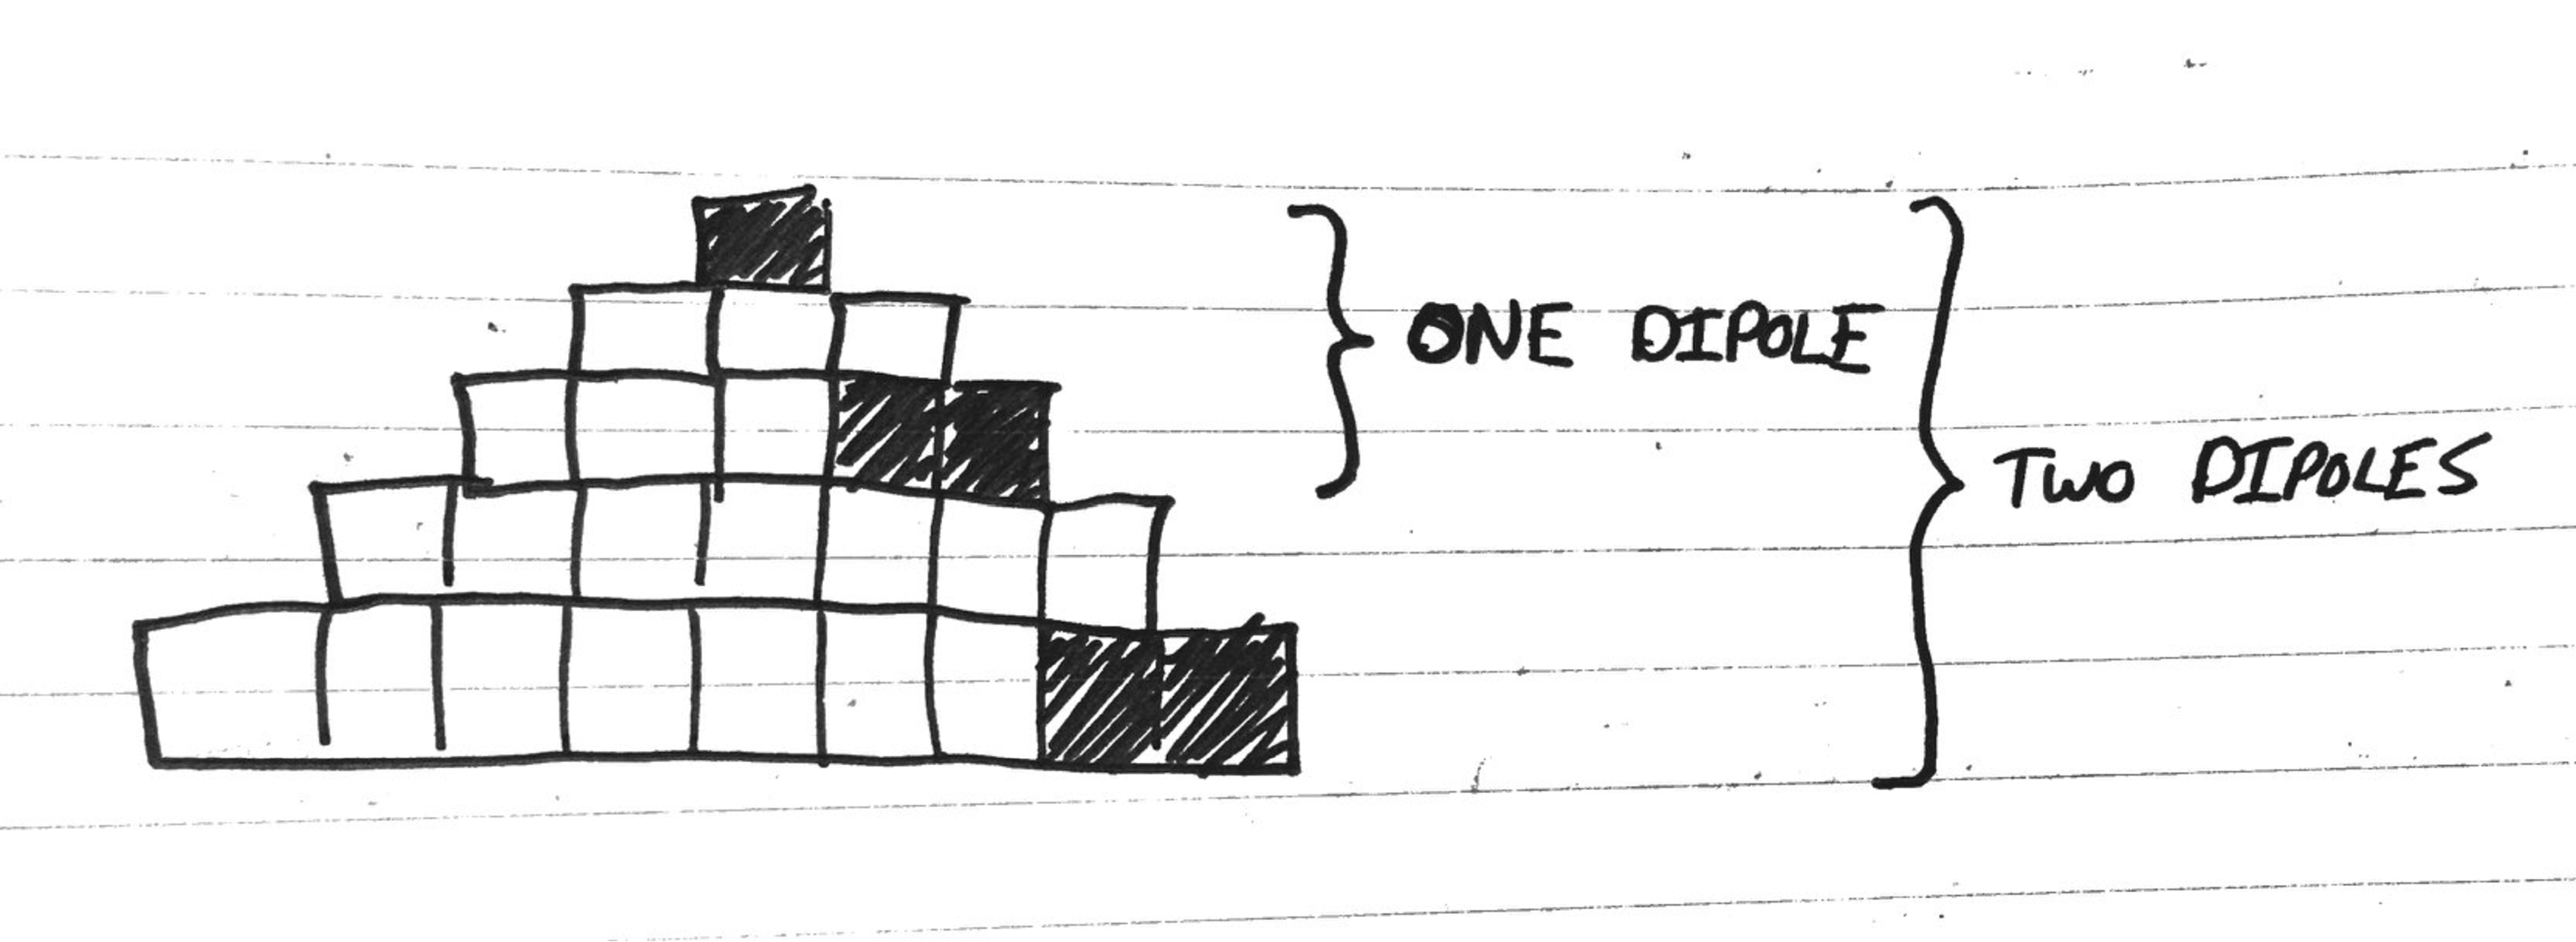
\includegraphics[width=0.8\textwidth, interpolate=true]{figs/minsamp}
\end{center}
M. Vetterli, P. Marziliano and T. Blu, "Sampling signals with finite rate of innovation," in IEEE Transactions on Signal Processing, vol. 50, no. 6, pp. 1417-1428, Jun 2002.\\
S. Deslauriers-Gauthier and P. Marziliano, "Sampling signals with a finite rate of innovation on the sphere," in IEEE Transactions on Signal Processing, vol. 61, no. 18, pp. 4552-4561, Sept.15, 2013.
\end{frame}
\begin{frame}[label=sec-12]{Giant Unilamallar Vesicles (GUV)\\ FOV $\approx$ 150 $\times$ 150 $\mu$\text{m}}
\begin{center}
  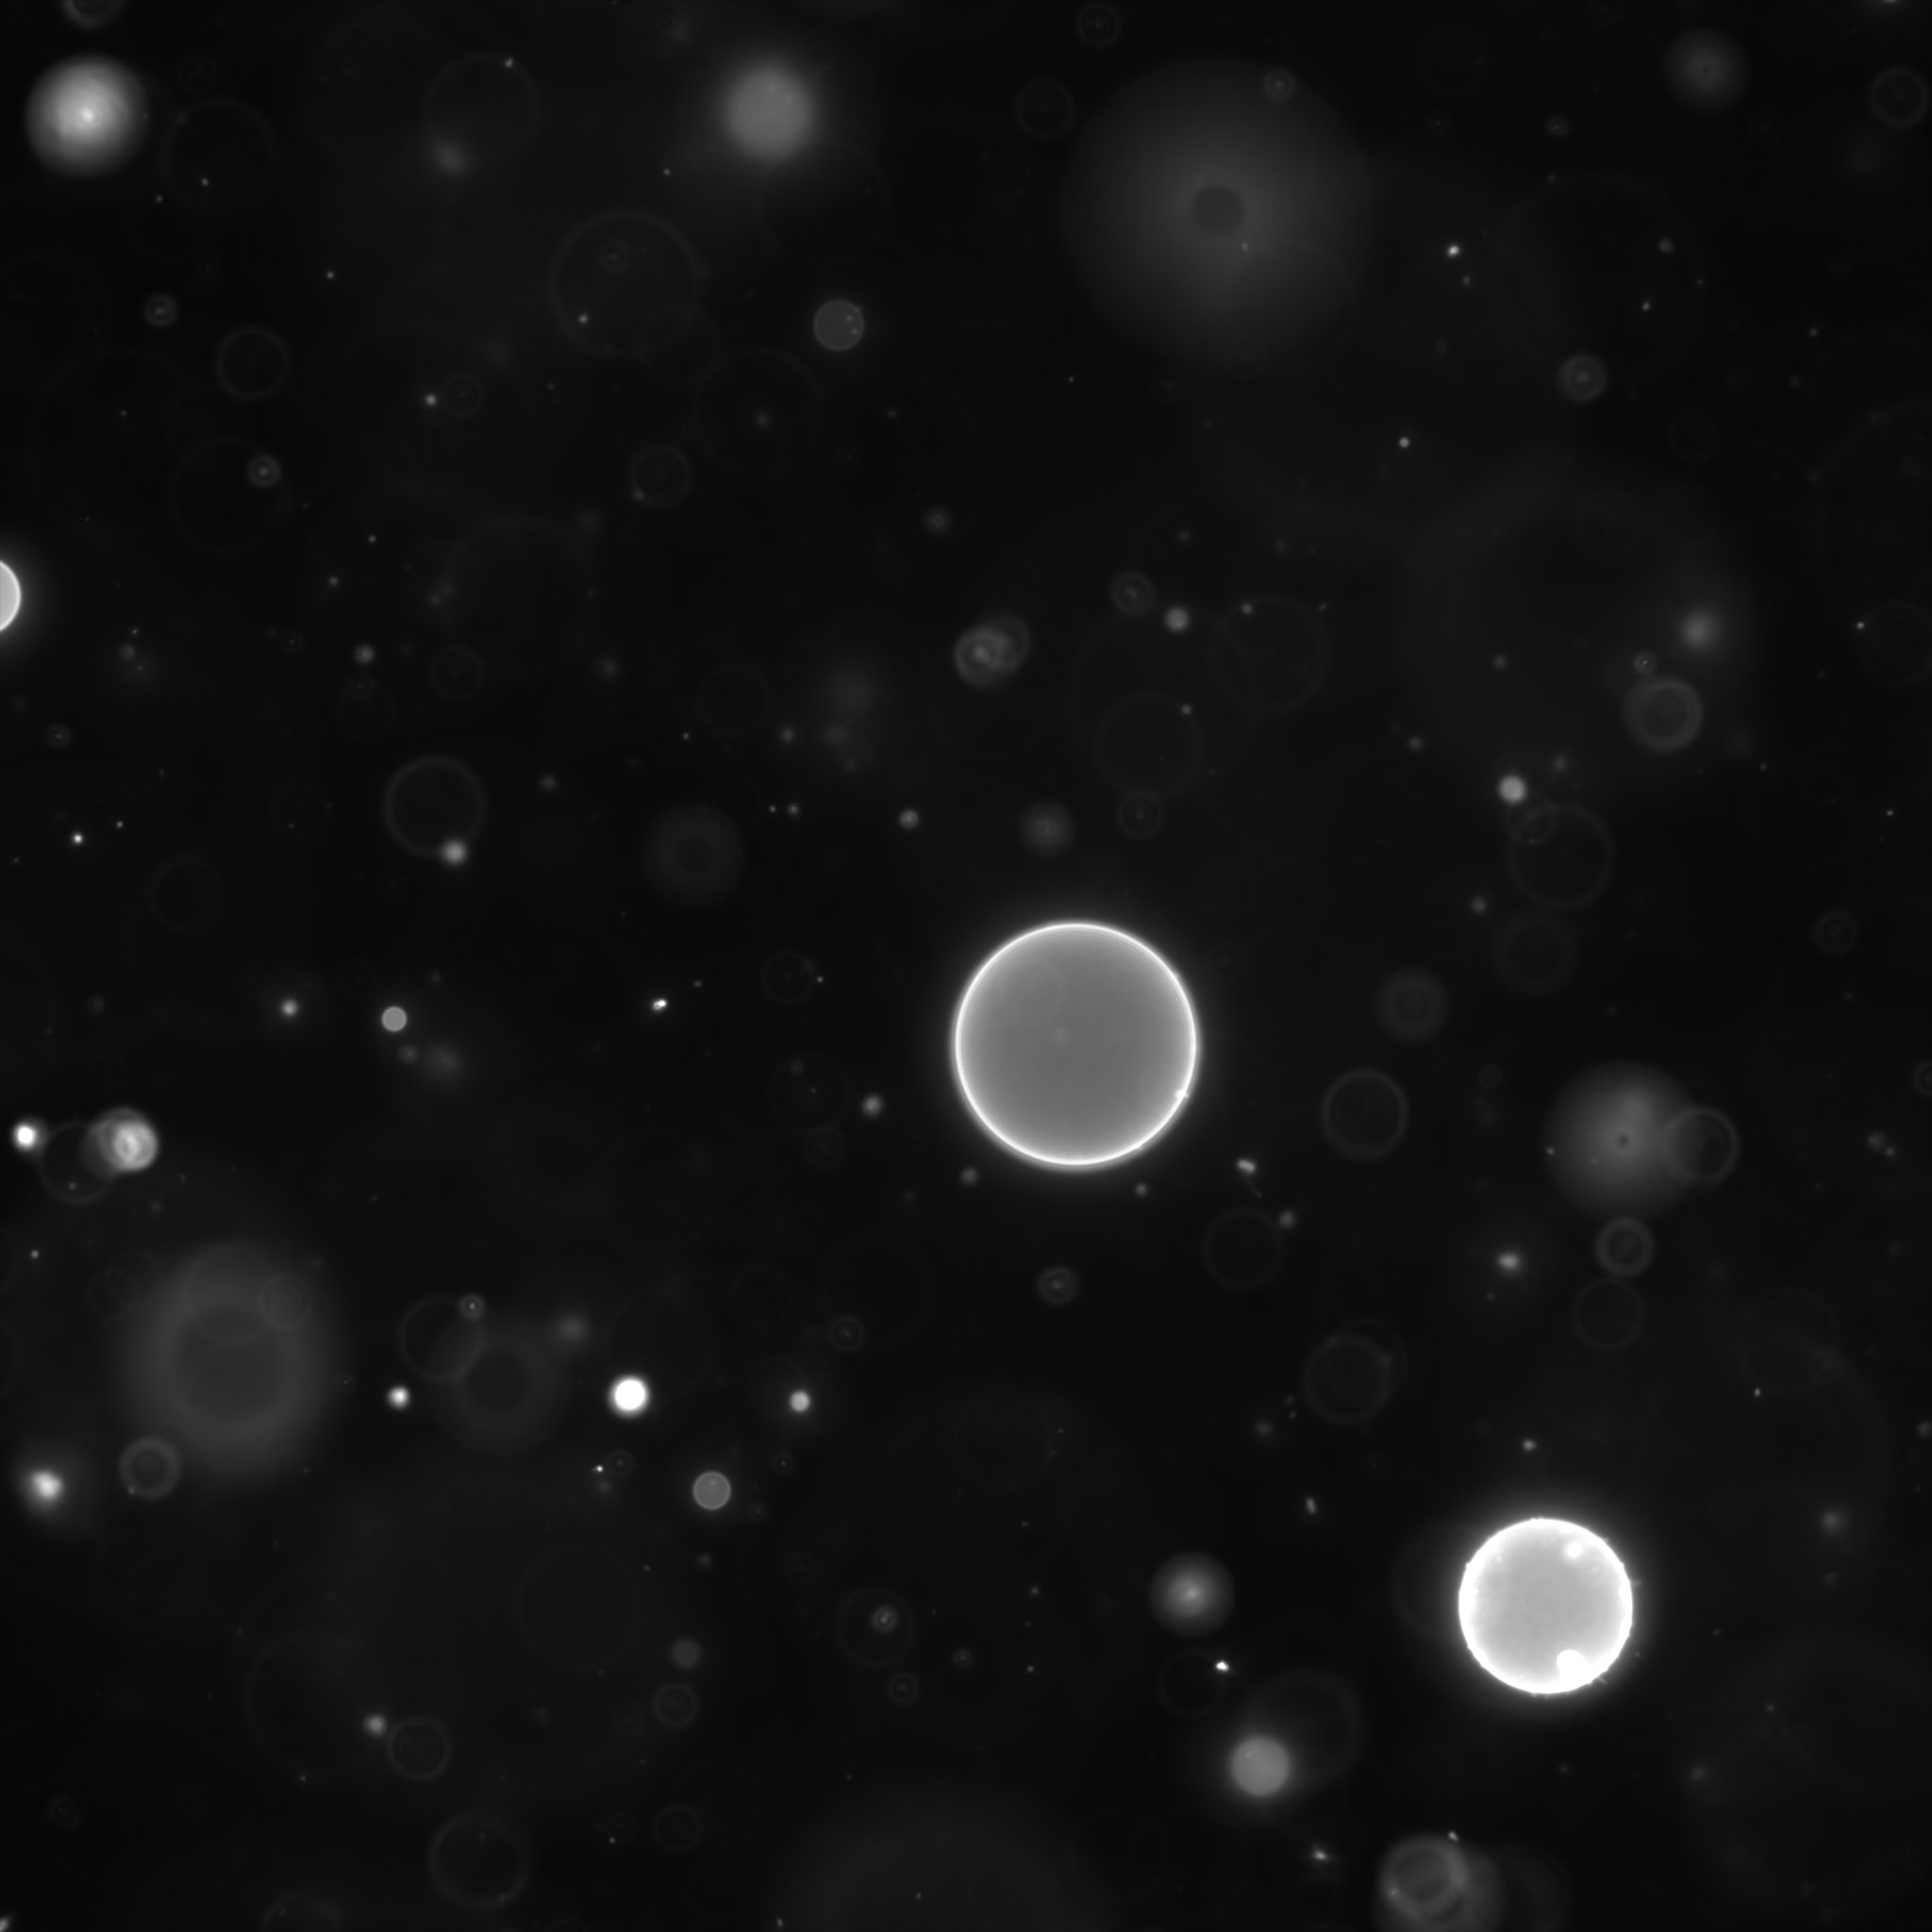
\includegraphics[width=0.6\textwidth, interpolate=true]{figs/guv.jpg}
\end{center}
\end{frame}
\begin{frame}[label=sec-13]{GUV Protocol}
\begin{center}
  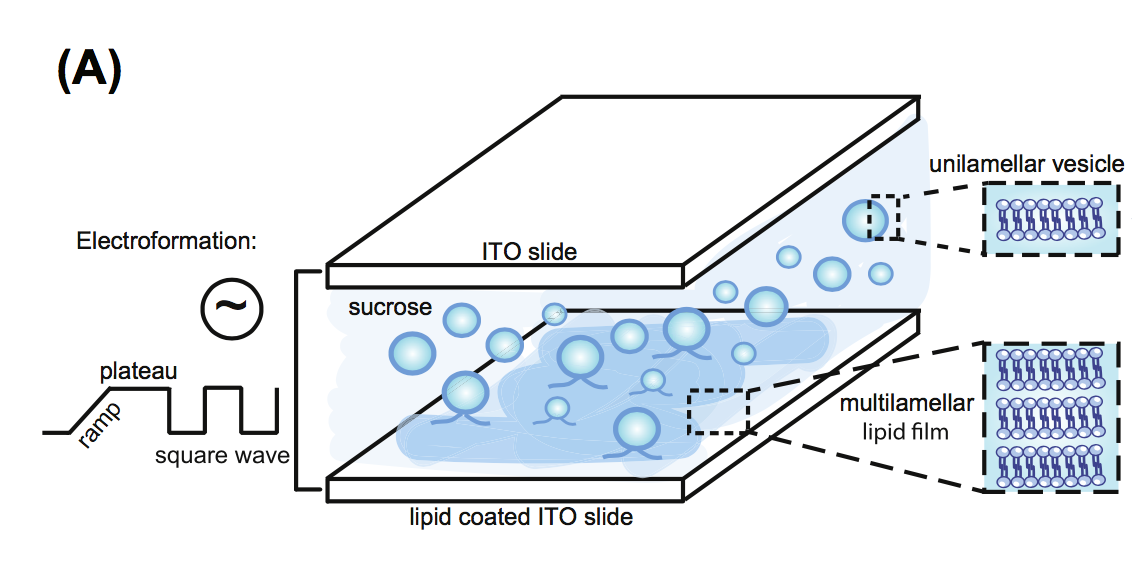
\includegraphics[width=0.9\textwidth, interpolate=true]{figs/schmid2015}
  \raisebox{-10pt}{\makebox[0pt][r]{\footnotesize Schmid, 2015}}
\end{center}
\end{frame}

\begin{frame}[label=sec-14]{GUV Chamber}
\begin{center}
  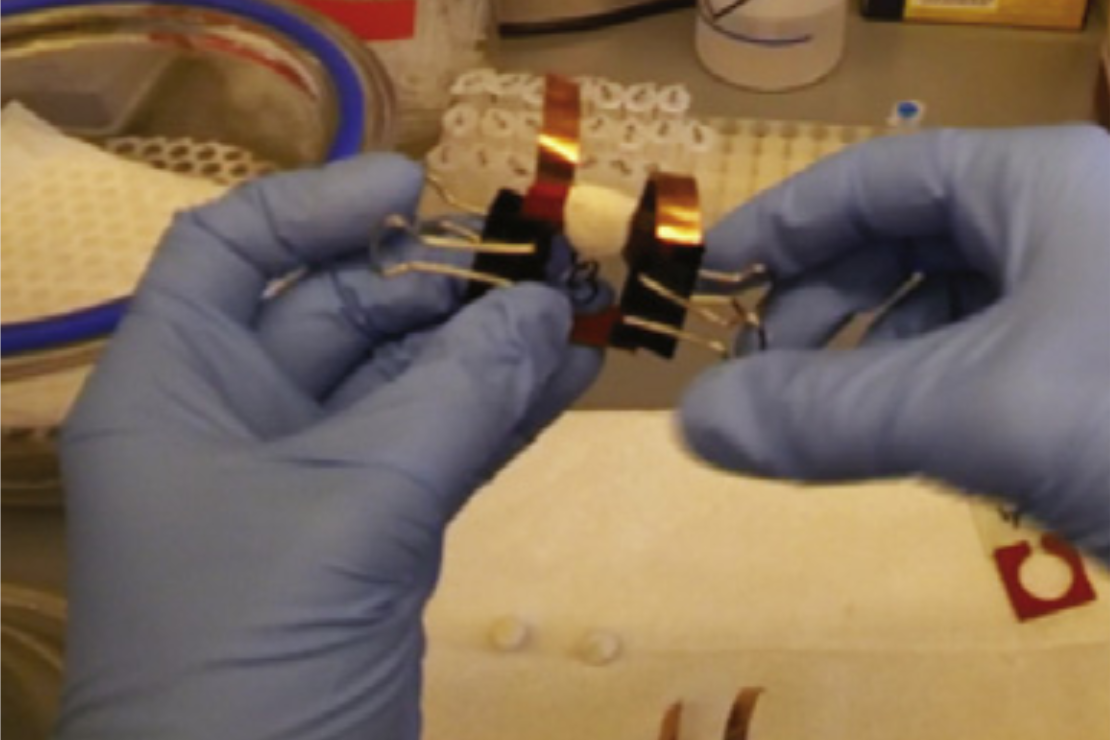
\includegraphics[width=0.7\textwidth, interpolate=true]{figs/chamber}
  \raisebox{-10pt}{\makebox[0pt][r]{\footnotesize Schmid, 2015}}
\end{center}
\end{frame}
% Emacs 25.3.1 (Org mode 8.2.10)
\end{document}